\begin{enumerate}[label=\thesection.\arabic*.,ref=\thesection.\theenumi]
\numberwithin{equation}{enumi}
\item The number of directions and encirclements around the point -1+j0 in the complex plane by the Nyquist plot of $G(s) = \frac{1-s}{4+2s}$\\

\solution
Substitute s = $\j\omega$ evaluate magnitude and phase at $\omega = 0$ and $\omega = \infty$

\begin{align}
G\brak{\j\omega} &= \frac{1-\j\omega}{4+2\j\omega} 
\end{align}


\begin{align}
\angle G\brak{\j\omega} &= \tan^{-1}(\frac{-\omega}{1}) - \tan^{-1}(\frac{\omega}{2})
\end{align}

so from this  at $\omega = 0$ $\angle G\brak{\j\omega} = 0$ 

and at $\omega = \infty$ $\angle G\brak{\j\omega}  =-180$  

\begin{align}
\abs{G\brak{\j\omega}} &= \frac{\sqrt{1+{\omega}^2}}{\sqrt{16+{4\omega}^2}} 
\end{align}

when $\omega = 0$ $\abs{G\brak{\j\omega}} = \frac{1}{4}$ 

and at  $\omega = \infty$ $\abs{G\brak{\j\omega}} = \frac{1}{2}$

Plot first 0.25 on positive x-axis then turn {-180} degrees from that point i.e {180} degrees clockwise(in this case).\\
Substitute $s = Re^{j\theta}$
\begin{align}
\lim_{R\to \infty}\,G\brak{Re^{\j\theta}} &= \frac{1-Re^{\j\theta}}{4+2Re^{\j\theta}}=\frac{-1}{2}  
\end{align}
As there are no $e^{\j\theta}$ terms.
There will be no enclosed Nyquist path here.
So, for this Transfer function $G(s)$,the Nyquist plot is the the Polar plot and its mirror image with respect to real axis.
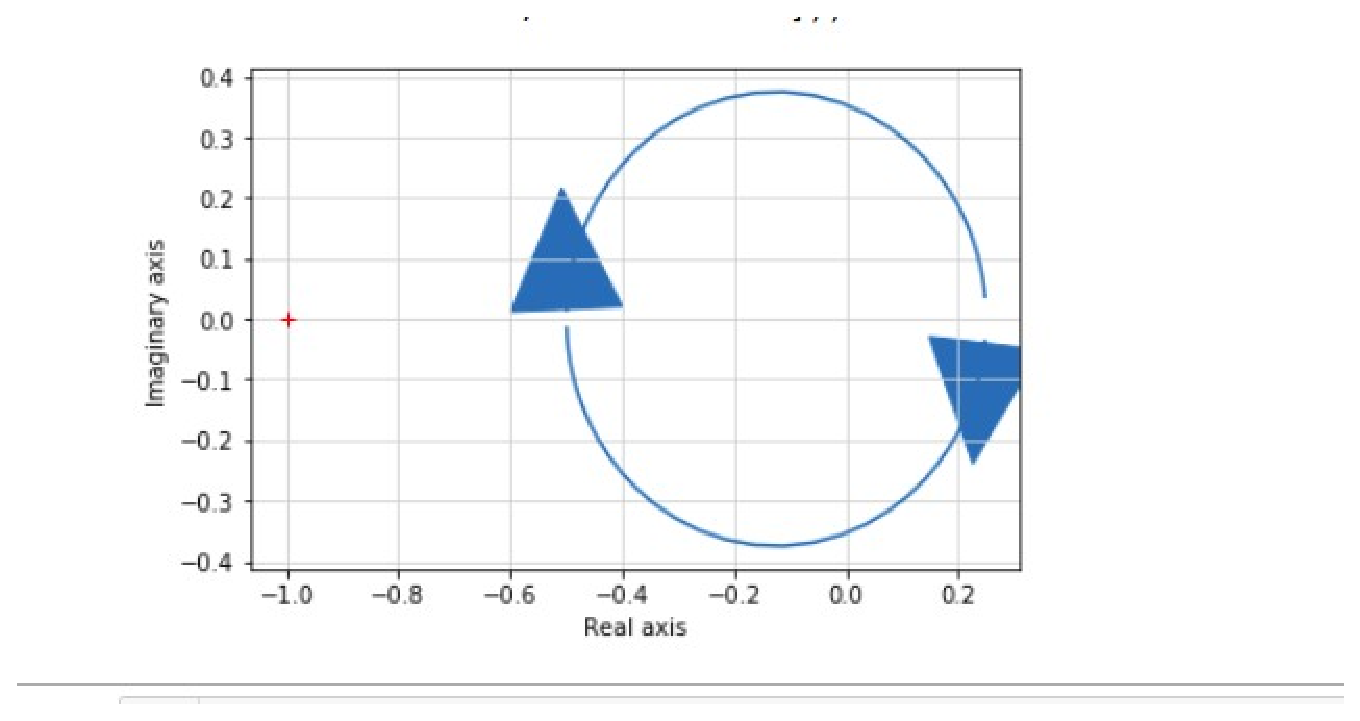
\includegraphics[width=\columnwidth]{./figs/pythonnyquistplot.eps}
As from the observed plot the co-ordinate -1 + j0 is outside the contour.

Hence,the number of encirclements around the the given co-ordinate is zero.
\end{enumerate}
